% IEEE conference paper. Compile on Overleaf (IEEEtran class and IEEEtran.bst are built in):
% upload the repo, set paper/main.tex as the main file. Figures come from ../figures/<stage>/<name>.pdf.
\documentclass[conference]{IEEEtran}
\usepackage{cite}
\usepackage{amsmath,amssymb}
\usepackage{graphicx}
\usepackage{booktabs}
\usepackage{multirow}
\usepackage{xcolor}
\usepackage[hidelinks]{hyperref}

\graphicspath{{../figures/}}
\newcommand{\ES}{\mathrm{ES}}
\newcommand{\VaR}{\mathrm{VaR}}
% Placeholder still to be filled in: renders in red so it cannot slip into the submitted version.
\newcommand{\fillin}[1]{\textcolor{red}{[#1]}}

\begin{document}

\title{Physics-Informed Neural Networks for\\ Financial Tail-Risk Estimation}

\author{
\IEEEauthorblockN{Aditya Siraskar, Utkarsh Sinha, Aditya Sharma}
\IEEEauthorblockA{\textit{\fillin{Department}, \fillin{Institute}}\\
\fillin{City}, India\\
\fillin{email addresses}}
}

\maketitle

\begin{abstract}
Value at Risk (VaR) and Expected Shortfall (ES) are properties of the tail of the loss distribution, which
under jump-diffusion dynamics is the solution of a forward partial integro-differential equation (PIDE). We
test whether physics-informed neural networks (PINNs) can supply this density accurately enough for tail risk,
against an exact ground truth at every step. A PINN with a log-density output, a log-form residual and
Gauss--Hermite quadrature of the jump integral recovers VaR and ES to within 1\% in one dimension; ablations
show that the log-form residual is essential, reducing 10-day ES errors from over 50\% to below 0.2\%. A
mesh-free extension with a coefficient-based importance proposal and a stochastic trace estimator keeps the
error near 1\% up to five assets at almost constant training cost, and breaks down at ten. An amortised network
over volatility level, jump intensity and jump mean covers a range of market states with one training run, but
Monte Carlo remains faster per query for the Merton model. On NIFTY and S\&P sector baskets (2018--2026) the PINN
reproduces its model's daily ES within 0.2--2.8\%, so its backtest performance is that of the model. Trained on
no samples, the PINN matches an identical network trained on $10^5$--$10^6$ exact samples. We also document where
the method fails, including a far-tail extrapolation failure and its remedy.
\end{abstract}

\begin{IEEEkeywords}
physics-informed neural networks, expected shortfall, value at risk, jump-diffusion, partial
integro-differential equations, importance sampling, backtesting
\end{IEEEkeywords}

% ================================================================================================
\section{Introduction}

Market-risk capital is set by the 97.5\% Expected Shortfall under the Basel Fundamental Review of the Trading
Book \cite{bcbs2019}, and ES is preferred to VaR because it is coherent \cite{artzner1999,acerbi2002}. Both are
tail quantities, and returns have fat tails, volatility clustering and jumps \cite{mandelbrot1963,cont2001}: a
model can fit the centre of the distribution and still misjudge the worst 1\%.

Jump-diffusion models \cite{merton1976,kou2002} capture these features. Their return density solves a forward
PIDE, from which VaR is a quantile and ES a tail integral. Finite differences solve this equation accurately, but
their cost grows as $n^d$ in $d$ assets \cite{andersen2000,cont2004}; Monte Carlo works in any dimension but
converges as $N^{-1/2}$ and must be rerun for every parameter set \cite{glasserman2003}. Physics-informed neural
networks \cite{raissi2019,karniadakis2021} are mesh-free, can take parameters as inputs, and are evaluated by a
forward pass.

PINNs have been applied to option pricing and to Fokker--Planck equations \cite{chen2021fp}, but whether a
PINN-solved density yields accurate and useful \emph{tail risk} has not been tested systematically. We ask when a
PINN gives better tail-risk estimates than conventional methods, and when its overhead outweighs the gain. The
contributions are:
\begin{itemize}
  \item a PINN design for the forward jump-diffusion PIDE that learns the tail as accurately as the bulk, with
        ablations of each component;
  \item a mesh-free $d$-asset extension in which collocation, normalisation and risk share one importance proposal
        built from the PIDE coefficients, scaled from one to ten assets;
  \item an amortised network over market parameters, with sensitivities by differentiation and an honest latency
        comparison with Monte Carlo;
  \item daily backtests on two real five-asset baskets in which the PINN error is separated from the model error;
  \item a physics-versus-data ablation that prices the equation in exact samples, and a set of failure cases.
\end{itemize}

% ================================================================================================
\section{Related Work}

\emph{Tail-risk estimation.} Standard approaches are parametric models with EWMA \cite{riskmetrics1996}, GARCH
\cite{bollerslev1986} or DCC \cite{engle2002} volatility; historical and filtered historical simulation
\cite{barone1999}; GARCH-filtered extreme value theory \cite{mcneil2000}; and Monte Carlo. VaR forecasts are
backtested by coverage \cite{kupiec1995} and independence \cite{christoffersen1998} tests. ES is not elicitable
alone \cite{gneiting2011}, but (VaR, ES) is jointly elicitable \cite{fissler2016}, which yields consistent scores
such as FZ0 \cite{patton2019}, compared by the Diebold--Mariano test \cite{diebold1995}.

\emph{Neural PDE solvers.} PINNs \cite{lagaris1998,raissi2019} minimise the PDE residual at sampled points.
Their training is fragile \cite{wang2021,krishnapriyan2021}. High-dimensional solvers include deep BSDE
\cite{han2018} and the deep Galerkin method \cite{sirignano2018}; Hutchinson's trace estimator
\cite{hutchinson1989} removes the $O(d)$ cost of the Laplacian in PINNs \cite{hu2024}. Neural operators
\cite{lu2021,li2021} learn parametric solution maps from solved examples, and normalising flows
\cite{papamakarios2021} learn densities from samples. Our amortised PINN learns a parametric density from the
equation alone, and our data-only baseline isolates what the equation adds.

% ================================================================================================
\section{Model and Method}

\subsection{Multi-Asset Jump-Diffusion}
Log returns $X_t \in \mathbb{R}^d$ follow a diffusion $\mathcal{N}(at, \Sigma t)$ plus a common market jump: at
Poisson($\lambda$) times all assets move by $\beta Y$ with $Y \sim \mathcal{N}(\mu_J, \sigma_J^2)$. The density
solves
\begin{equation}
  p_t = -a\cdot\nabla p + \tfrac12\operatorname{tr}(\Sigma\nabla^2 p)
        + \lambda\!\int\! p(x-\beta y,t)\,f_Y(y)\,dy - \lambda p .
  \label{eq:pide}
\end{equation}
The jump integral is one-dimensional for any $d$, and the exact density is a Poisson mixture of Gaussians
\cite{merton1976}, so every error below is measured against an exact value. For a linear portfolio $w$,
$w^\top X$ is a 1-D Merton process, which gives exact VaR and ES for every portfolio.

\subsection{PINN Design}
The network outputs the log density with the known Gaussian normaliser added,
$u = -\tfrac12\log\det(2\pi\Sigma t) + c\,g_\phi(z,\tau)$, with whitened similarity input
$z = L^{-1}(x - at)/\sqrt{t}$ ($LL^\top = \Sigma$) and scaled $\log t$. Dividing \eqref{eq:pide} by $p$ gives the
\emph{log-form residual}
\begin{equation}
  r = u_t + a\cdot\nabla u - \tfrac12\big[\operatorname{tr}(\Sigma\nabla^2 u) + \nabla u^\top\Sigma\nabla u\big]
      - \lambda (S-1),
\end{equation}
with $S = \int e^{u(x-\beta y)-u(x)} f_Y(y)\,dy$ computed by 48-node Gauss--Hermite quadrature. The residual measures
relative error, so a tail point weighs as much as a bulk point; the standard residual on $p$ weights it by its tiny
density. The trace is exact for $d \le 4$ and estimated with four Rademacher probes \cite{hutchinson1989} above.
Training starts at $t_0 = 0.5$ day from the exact density, which avoids the Dirac delta at $t = 0$. The loss is
$\overline{(t r)^2} + 10\,\overline{(u - u_0)^2}_{t_0} + 10\,\overline{(\log \hat m)^2}$, where $\hat m$ is an
importance-sampling estimate of $\int p\,dx$ (the log residual is blind to scaling $p$). We use Adam with a cosine
schedule from $2\times10^{-3}$ for 20{,}000 steps.

\subsection{Coefficient-Based Proposal and Risk}
Without a grid, collocation, normalisation and risk all draw from
\begin{equation}
  q(x\mid t) = \sum_{k=0}^{K}\pi_k\, t_\nu\!\big(x;\, at + k\mu_J\beta,\; c^2(\Sigma t + k\sigma_J^2\beta\beta^\top)\big),
\end{equation}
a Student-$t$ mixture over jump counts with floored Poisson weights, built from the PIDE coefficients only. VaR and
ES of any portfolio are the weighted quantile and tail mean of self-normalised importance weights
$\propto e^{u - \log q}$; one set of draws serves every portfolio, and Euler contributions $\partial\ES/\partial w_i$
follow from the same draws. A trust region gives zero weight to draws more than six radii from the training region.

\subsection{Amortised Model and Data-Only Baseline}
The amortised network adds $\theta = (s, \lambda, \mu_J)$ as inputs, where $s$ scales all volatilities, and draws a
fresh $\theta$ for every training point from $s\in[0.6,1.6]$, $\lambda\in[1,15]$/yr, $\mu_J\in[-0.10,-0.02]$. The
data-only baseline is the identical network, optimiser, schedule and normaliser, trained instead by maximum
likelihood on $N$ exact samples over 16 times, with 20\% held out for early stopping.

% ================================================================================================
\section{Experimental Setup}

Base parameters are $a = 0.05$, $\lambda = 5$/yr, $\mu_J = -0.05$, $\sigma_J = 0.07$; the $d$-asset family has
volatilities in $[0.18, 0.30]$, loadings in $[0.8, 1.2]$ and correlation 0.4. The headline metric is the relative
ES$_{99}$ error at 1, 5 and 10 days, median over 20 portfolios. Every comparison includes the same estimator with the
exact density (the sampling floor) and Monte Carlo at the same budget ($2^{18}$ draws), on common random numbers.

The real-data study uses five-asset baskets of NIFTY stocks (Reliance, HDFC Bank, Infosys, ICICI Bank, TCS) and S\&P
sector ETFs (XLK, XLF, XLE, XLV, XLI), developed on 2006--2017 and tested on 2018--2026 (about 2{,}200 days). The
model is fitted by maximum likelihood with a daily EWMA volatility scale and monthly shrinkage recalibration of
$(\lambda, \mu_J)$. Benchmarks are Gaussian, historical simulation (HS), filtered HS (FHS), GARCH-$t$, GARCH-EVT,
DCC-GARCH-$t$ and unfiltered Merton. All training runs on one NVIDIA T4 GPU with under 0.5\,GB of memory.

% ================================================================================================
\section{Results}

\subsection{One Dimension and Ablations}
The 1-D PINN recovers every VaR and ES from 95\% to 99.9\% within 1\% (ES$_{99}$: 0.30/0.42/0.16\% at 1/5/10 days)
after 8.6 minutes of training. Table~\ref{tab:ablation} removes one component at a time. The log-form residual is
essential, quadrature resolution sets the short-horizon error, and tail-adaptive sampling gives no gain. Finite
differences remain faster and more accurate in 1-D.

\begin{table}[t]
  \caption{1-D Ablations: ES$_{99}$ Error, Range Over Three Seeds}
  \label{tab:ablation}
  \centering
  \begin{tabular}{lcc}
    \toprule
    Variant & 1 day & 10 days \\
    \midrule
    Full design                 & 0.18--0.30\% & 0.06--0.16\% \\
    Residual on $p$             & 0.9--22\%    & 57--152\% \\
    8 quadrature nodes          & 12--15\%     & 0.2--0.8\% \\
    No normalisation penalty    & 2.1--2.2\%   & 0.07--0.14\% \\
    No tail-adaptive sampling   & 0.06--0.36\% & 0.04--0.05\% \\
    \bottomrule
  \end{tabular}
\end{table}

\subsection{Scaling With Dimension}
Table~\ref{tab:scaling} and Fig.~\ref{fig:scaling} show that the error stays near 1\% up to $d = 5$ with training
time almost flat in $d$, a regime where a 2-D finite-difference grid already takes 55\,s against 0.3\,s in 1-D.
At $d = 10$ the PDE loss stalls and the density is too wide along $\beta$, giving 62\% error at 10 days. We report
$d = 10$ as the breakdown point of this architecture and budget.

\begin{table}[t]
  \caption{Scaling: Median ES$_{99}$ Error at 1 Day / 10 Days}
  \label{tab:scaling}
  \centering
  \begin{tabular}{lccc}
    \toprule
    $d$ & PINN & Monte Carlo (same $N$) & Train (min) \\
    \midrule
    1  & 1.4\% / 0.05\% & 1.1\% / 0.22\% & 9.4 \\
    2  & 0.7\% / 1.0\%  & 1.4\% / 1.6\%  & 10.5 \\
    5  & 1.1\% / 0.6\%  & 0.2\% / 0.4\%  & 12.8 \\
    10 & 5.2\% / 62\%   & 0.6\% / 0.8\%  & 13.3 \\
    \bottomrule
  \end{tabular}
\end{table}

\begin{figure}[t]
  \centering
  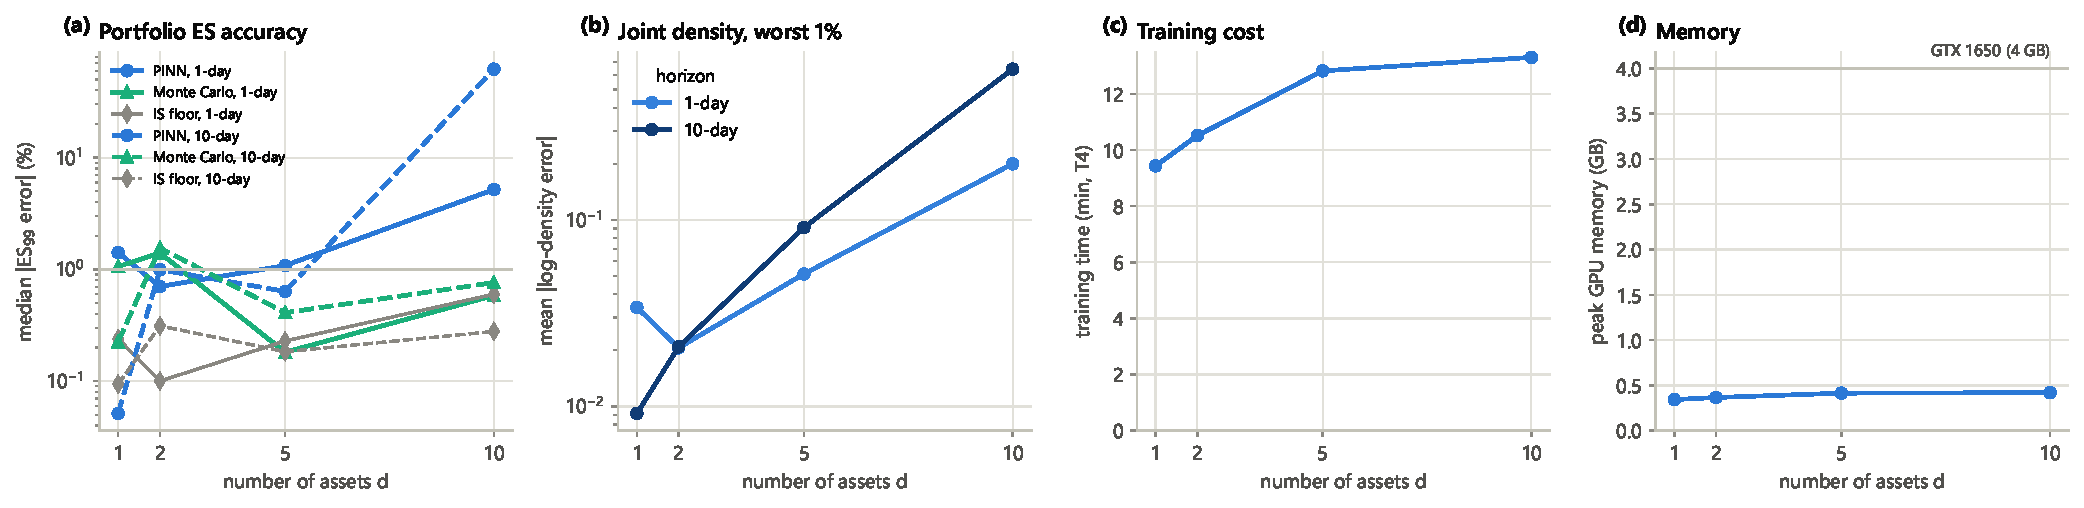
\includegraphics[width=\linewidth]{stage4_summary/fig01_scaling.pdf}
  \caption{ES$_{99}$ error against dimension: PINN, Monte Carlo at the same budget and the sampling floor.}
  \label{fig:scaling}
\end{figure}

\subsection{Amortised Real-Time Risk}
One amortised network (18--22 minutes of training) gives a median ES$_{99}$ error of 1.3/0.8/0.7\% at $d = 2$ over
the parameter grid, against 1.8/0.9/0.8\% for Monte Carlo at the same $N$. At $d = 5$ it reaches 3.4\% at 10 days
and 10\% in the worst corner. Euler contributions agree with finite differences of the exact ES within about 5\%.
Monte Carlo is nevertheless faster at matched error (0.9--1.6\,ms against 4--18\,ms per query), so there is no
break-even: exact Merton simulation is as cheap as drawing from the proposal.

\subsection{Real-Data Backtests}
Against its own model evaluated with the exact density on the same draws, the PINN's daily ES error has median
2.8\% (NIFTY) and 0.2\% (S\&P) at 99\%, with identical breaches, at 8.7\,ms per day. Table~\ref{tab:backtest}
therefore measures the model. It passes Kupiec at 99\% on both markets and beats Gaussian, HS and unfiltered Merton
on FZ0, but ranks behind volatility-filtered models with fat-tailed innovations, and it is conservative at 97.5\%.

\begin{table}[t]
  \caption{99\% Backtests, Linear Basket, 2018--2026 (FZ0: Lower Is Better)}
  \label{tab:backtest}
  \centering
  \setlength{\tabcolsep}{4pt}
  \begin{tabular}{lcccc}
    \toprule
    & \multicolumn{2}{c}{NIFTY} & \multicolumn{2}{c}{S\&P} \\
    Model & Breaches & FZ0 & Breaches & FZ0 \\
    \midrule
    DCC-GARCH-$t$ & 28 & $-3.301$ & 33 & $-3.294$ \\
    Filtered HS   & 19 & $-3.278$ & 20 & $-3.244$ \\
    GARCH-EVT     & 26 & $-3.201$ & 20 & $-3.353$ \\
    \textbf{PINN} & 15 & $-3.156$ & 27 & $-3.046$ \\
    Merton (exact)& 15 & $-3.134$ & 27 & $-3.044$ \\
    HS            & 26 & $-3.016$ & 30 & $-2.731$ \\
    Gaussian      & 38 & $-2.881$ & 59 & $-2.297$ \\
    \bottomrule
  \end{tabular}
\end{table}

\subsection{Physics Versus Data}
Table~\ref{tab:physdata} and Fig.~\ref{fig:physdata} compare the PINN, trained on no samples, with the identical
network trained on $N$ exact samples. The data-only network needs $10^5$--$10^6$ samples to match the PINN, and at
realistic sizes ($10^3$--$10^4$) its errors are 5--60\%. Results at $d = 5$ are similar.

\begin{table}[t]
  \caption{Physics Versus Data, $d = 2$: Median ES$_{99}$ Error}
  \label{tab:physdata}
  \centering
  \begin{tabular}{lccc}
    \toprule
    Method & 1 day & 5 days & 10 days \\
    \midrule
    \textbf{PINN (no samples)} & \textbf{1.3\%} & \textbf{0.9\%} & \textbf{0.08\%} \\
    Data-only, $N = 10^4$ & 13\%  & 2.1\% & 3.8\% \\
    Data-only, $N = 10^5$ & 5.0\% & 0.8\% & 2.5\% \\
    Data-only, $N = 10^6$ & 1.3\% & 0.4\% & 0.18\% \\
    Monte Carlo, same $10^6$ & 0.8\% & 1.2\% & 1.1\% \\
    \bottomrule
  \end{tabular}
\end{table}

\begin{figure*}[t]
  \centering
  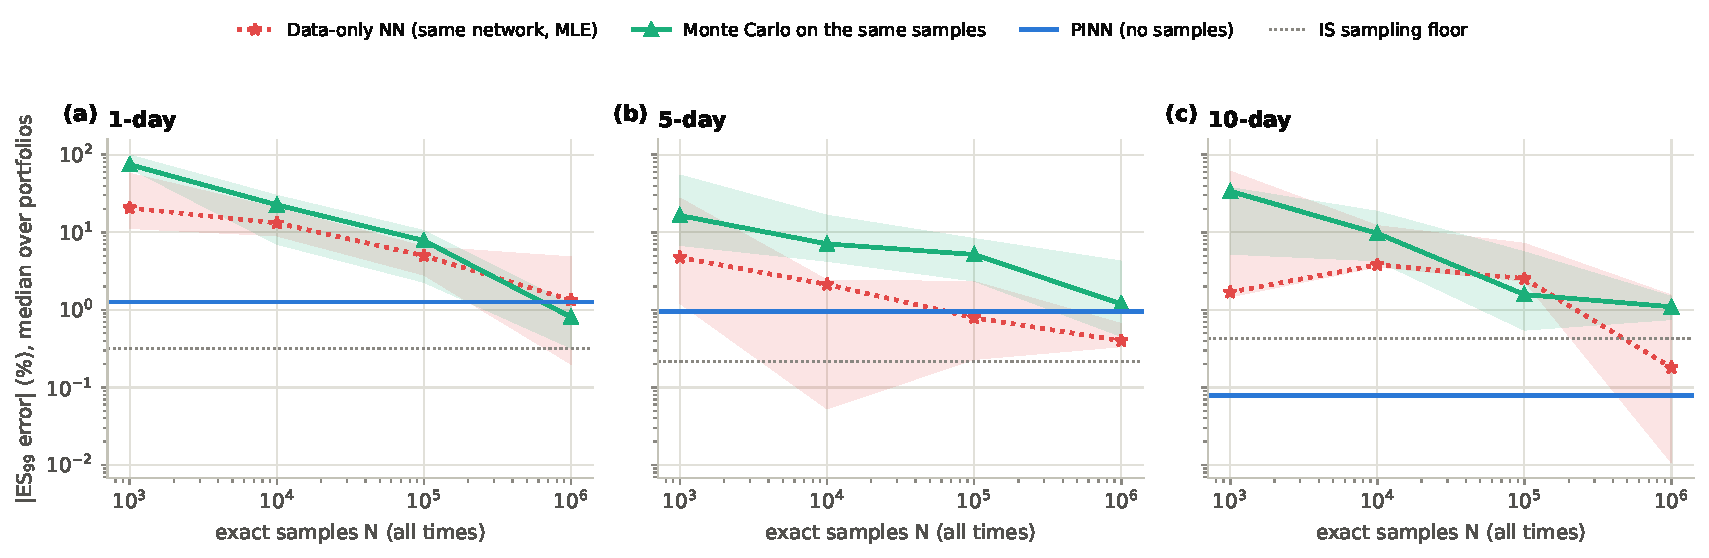
\includegraphics[width=0.9\textwidth]{stage7_physics_vs_data_d2/fig02_es_vs_samples.pdf}
  \caption{ES$_{99}$ error against the number of exact samples ($d = 2$): data-only network (red), Monte Carlo on the
    same samples (green), and the PINN, which uses none (blue).}
  \label{fig:physdata}
\end{figure*}

\subsection{Failure Cases}
A crisis jump rate ($\lambda = 50$/yr) with a proposal covering only three jumps degrades the error only to 0.8\%,
and widening the proposal to ten jumps restores 0.1\%. A start time ten times closer to $t = 0$ fails at short
horizons (5.2\% ES and 21\% VaR error at 1 day) and recovers by 10 days. The far-tail probe in
Fig.~\ref{fig:failure}(b) explains a real-data failure: outside its training region the PINN's log density decays
more slowly than the heavy-tailed proposal, so a single far draw can take all the importance weight. This occurred
once on the S\&P basket (2022-06-16) and is removed by the trust region.

\begin{figure*}[t]
  \centering
  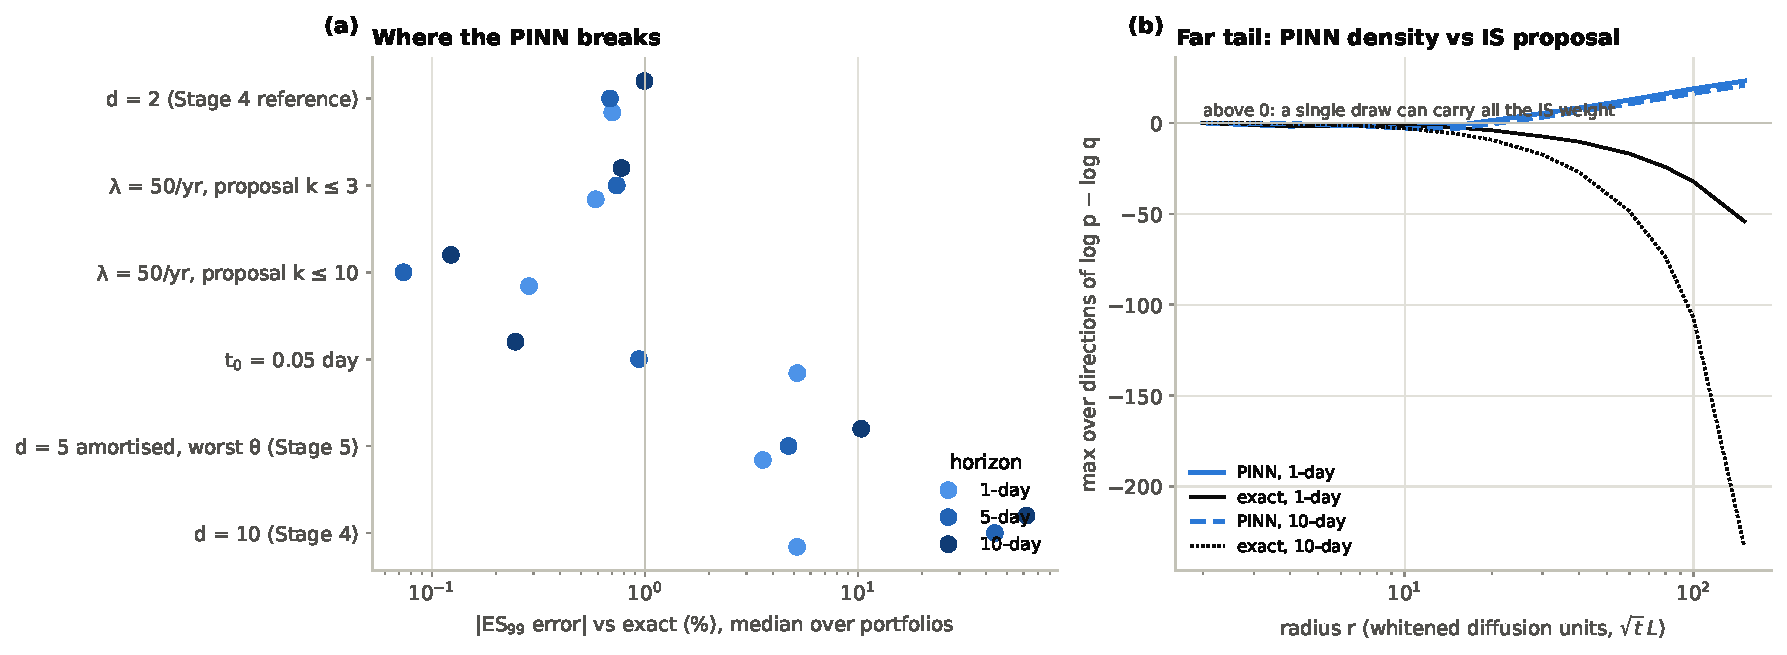
\includegraphics[width=0.9\textwidth]{stage7_final/fig02_failure_cases.pdf}
  \caption{(a) ES$_{99}$ error by failure case and horizon. (b) Maximum over 2{,}000 directions of $\log p - \log q$
    for the PINN and the exact density: the PINN turns positive beyond about 20 whitened units.}
  \label{fig:failure}
\end{figure*}

% ================================================================================================
\section{Discussion}

The design matters more than the network: the log-form residual, the quadrature resolution and the normalisation
each change the tail error by an order of magnitude. The equation is worth $10^5$--$10^6$ samples, which is decisive
when data are scarce. Speed, however, is not the selling point for a model as cheap to simulate as Merton; the
PINN's value is a smooth, normalised and differentiable density over times and parameters, useful for
sensitivities, scenarios and models that are expensive to simulate. On real data the PINN reproduces whatever model
it is given, so better tail forecasts require better models rather than better networks. Finally, a neural density
must not be trusted outside its training region.

\emph{Limitations.} The study uses one common jump factor, volatility only as a daily scale, and the exact
short-time density as initial condition; the method was not made to work at ten assets.

% ================================================================================================
\section{Conclusion}

A carefully designed PINN learns jump-diffusion tails to about 1\% ES error up to five assets, scales at nearly
constant cost, and replaces $10^5$--$10^6$ samples of data, but for the Merton model it does not beat Monte Carlo on
latency, and on real data its accuracy is bounded by the model it solves. Future work includes stochastic
volatility and self-exciting jumps, where simulation is expensive; time-marching and low-rank networks beyond ten
assets; and uncertainty estimates that flag extrapolation automatically. Code, configurations and all results are
available at \url{https://github.com/aditya-siraskar/PINN_FTRE}.

\bibliographystyle{IEEEtran}
\bibliography{references}

\end{document}
